\chapter{Numerical methods for diffusion problems}

\section{Introduction: boundary value problems}

Consider the following problem:

\begin{equation}
\begin{cases}
    \Lcur u = f & \text{in } \Omega \\
    \text{B.C.} & \text{on } \partial \Omega
\end{cases}
\end{equation}

where:
\begin{itemize}
    \item $\Omega \subset \R^d$ is an open bounded domain, with $d = 2, 3$
    \item $\partial \Omega$ is the boundary of $\Omega$
    \item $f$ given function
    \item Boundary conditions (BC) to be prescribed according to $\Lcur$
    \item $\Lcur$ a 2nd order differential operator
\end{itemize}

\begin{example}
    \begin{enumerate}
        \item $\Lcur u = -\dv(\mu \nabla u) + \mathbf{b} \cdot \nabla u + \sigma u$ (non-conservative form)
        \item $\Lcur u = -\dv(\mu \nabla u) + \dv(\mathbf{b} u) + \sigma u$ (conservative form)
    \end{enumerate}

    with $\mu \in L^{\infty}(\Omega), \mu(x) \geq \mu_0 > 0$, $\mathbf{b} \in (L^{\infty}(\Omega))^d$, $\sigma, f \in L^{2}(\Omega)$.
\end{example}

We may propose the following boundary conditions:

\begin{equation}
    \begin{cases}
        u = 0 & \text{on } \Gamma_D \\
        \mu \nabla u \cdot \mathbf{n} = g & \text{on } \Gamma_N
    \end{cases}
\end{equation}

Where $g \in L^2(\Gamma_D)$, $\partial \Omega = \Gamma_D \cup \Gamma_N$, $\Gamma_D \cap \Gamma_N = \emptyset$. We call 
$\Gamma_D$ the Dirichlet boundary and $\Gamma_N$ the Neumann boundary.

\begin{figure}[H]
    \centering
    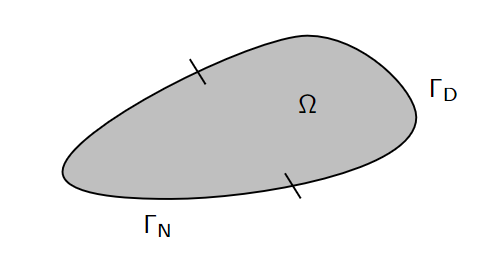
\includegraphics[width=0.5\textwidth]{figures/dirich_neum_bound.png}
    \caption{Representation of Dirichlet and Neumann boundary}
    \label{fig:dirich_neum_bound}
\end{figure}

So in general, let us focus on the following problem:

\begin{equation}
    \begin{cases}
        -\dv(\mu \nabla u) + \mathbf{b} \cdot \nabla u + \sigma u = f & \text{in } \Omega \\
        u = 0 & \text{on } \Gamma_D \\
        \mu \nabla u \cdot \mathbf{n} = g & \text{on } \Gamma_N
    \end{cases}
\end{equation}

To solve this problem, it is useful to change the way it is formulated.


\section{Weak formulation}

The idea behind the weak formulation is as follows:

\begin{enumerate}
    \item Multiply the equation by a test function $v \in V$ (we don't know $V$ yet)
    
    $$\left( -\dv(\mu \nabla u) + \mathbf{b} \cdot \nabla u + \sigma u \right) v = f v $$

    \item Integrate over $\Omega$
    
    $$\int_{\Omega} \left( -\dv(\mu \nabla u) + \mathbf{b} \cdot \nabla u + \sigma u \right) v \, dx = \int_{\Omega} f v \, dx$$

    \item Integrate by parts
    
    $$\int_{\Omega} \mu \nabla u \cdot \nabla v \, dx - \int_{\partial \Omega} \mu \nabla u \cdot \mathbf{n} v \, ds + \int_{\Omega} \mathbf{b} \cdot \nabla u v \, dx + \int_{\Omega} \sigma u v \, dx = \int_{\Omega} f v \, dx$$
\end{enumerate}

Note that, for the boundary terms, we have:

$$\int_{\partial \Omega} \mu \nabla u \cdot \mathbf{n} v \, ds = \int_{\Gamma_D} \mu \nabla u \cdot \mathbf{n} v \, ds
+ \int_{\Gamma_N} \mu \nabla u \cdot \mathbf{n} v \, ds$$

and, if we impose that $v = 0$ on $\Gamma_D$, then the first term is zero. So we have:

$$\int_{\partial \Omega} \mu \nabla u \cdot \mathbf{n} v \, ds = \int_{\Gamma_N} g v \, ds$$

where $g = \mu \nabla u \cdot \mathbf{n}$, by the Neumann boundary condition. We rewrite the equation as:

$$
    \underbrace{\color{red}\int_{\Omega} \mu \nabla u \cdot \nabla v \, dx + 
    \int_{\Omega} \mathbf{b} \cdot \nabla u v \, dx + \int_{\Omega} \sigma u v \, dx}_{\color{red}a(u, v)} 
    = \underbrace{\color{blue}\int_{\Omega} f v \, dx + \int_{\Gamma_N} g v \, ds}_{\color{blue}F(v)}
$$

\begin{equation}
    \Longrightarrow \; {\color{red}a(u, v)} = {\color{blue}F(v)}
\end{equation}

We still need to define the space $V$. We will define it as:

$$V = \{ v \in H^1(\Omega) \; | \; v = 0 \text{ on } \Gamma_D \}$$

where $H^1(\Omega)$ is the Sobolev space, formally defined as:

\begin{fdefinition}
    Let $\Omega \subset \R^d$ be an open bounded domain. The \textbf{Sobolev space} $H^1(\Omega)$ is defined as:

    $$H^1(\Omega) = \{ v \in L^2(\Omega) \; | \; \nabla v \in (L^2(\Omega))^d \}$$

    where $\nabla v = (\partial_1 v, \ldots, \partial_d v)$. The norm in $H^1(\Omega)$ is defined as:

    $$\norm{v}_{H^1(\Omega)} = \left( \norm{v}_{L^2(\Omega)}^2 + \norm{\nabla v}_{L^2(\Omega)}^2 \right)^{1/2}$$

\end{fdefinition}

Then, notice that $V$ is just a subspace of $H^1(\Omega)$, where we impose the Dirichlet boundary condition.
We will use the following notation:

\begin{equation}
    H_{\Gamma_D}^1(\Omega) = \{ v \in H^1(\Omega) \; | \; v = 0 \text{ on } \Gamma_D \}
\end{equation}

Thus, the weak formulation of the problem, given the space $V$, is:

\begin{fdefinition}[Abstract weak formulation]
    Find $u \in V$ such that:

    $$a(u, v) = F(v) \quad \forall v \in V$$

    where $a: V \times V\to \R$ is a bilinear form and 
    $F: V \to \R$ is a linear form, both defined as (1.4)
\end{fdefinition}

How do we know that the problem has a solution? We need to prove the existence and uniqueness of the solution,
by using the Lax-Milgram theorem.

\subsection{Lax-Milgram theorem}

\begin{ftheorem}[Lax-Milgram]
    Let $V$ be a Hilbert space, $a: V \times V \to \R$ a bilinear form, and $F: V \to \R$ a linear form.
    Assume that:

    \vspace{1em}
    \begin{enumerate}[label=(\roman*)]
        \item $V$ is a Hilbert space with inner product $\intprod{\cdot}{\cdot}$ and norm $\norm{\cdot}_V$.
        
        \vspace{1em}

        \item $F \in V'$, where $V'$ is the dual space of $V$ (i.e., $F$ is bounded).
        
        \vspace{1em}

        \item $a$ is continuous, i.e., $\exists M > 0$ s.t.:
            $$|a(u, v)| \leq M \norm{u}_V \norm{v}_V \quad \forall u, v \in V$$

        \item $a$ is coercive, i.e., $\exists \alpha > 0$ s.t.:
            $$a(u, u) \geq \alpha \norm{u}_V^2 \quad \forall u \in V$$
            
    \end{enumerate}

    Then, there exists a unique solution $u \in V$ to the weak formulation problem. Moreover, the solution satisfies:

    $$\norm{u}_V \leq \frac{1}{\alpha} \norm{F}_{V'}$$

\end{ftheorem}

\begin{example}[\textbf{Diffusion equation}]
    Let us consider the following problem:

    \begin{equation}
        \begin{cases}
            -\dv(\mu \nabla u) = f & \text{in } \Omega \\
            u = 0 & \text{on } \partial \Omega = \Gamma_D \\
        \end{cases}
    \end{equation}

    We can write the weak formulation as:

    $$a(u, v) = \int_{\Omega} \mu \nabla u \cdot \nabla v \, dx, \quad F(v) = \int_{\Omega} f v \, dx$$

    with $V = H_{\Gamma_D}^1(\Omega)$. We need to prove that the Lax-Milgram theorem holds for this problem:\\

    \begin{enumerate}[label=(\roman*)]
        \item $V$ is a Hilbert space, since $H_{\Gamma_D}^1(\Omega)$ is a closed subspace of $H^1(\Omega)$.
        
        \item $F \in V'$, since:
        $$|F(v)| \leq \norm{f}_{L^2(\Omega)} \norm{v}_{L^2(\Omega)} \leq \norm{f}_{L^2(\Omega)} \norm{v}_V$$

        \item $a$ is continuous, since:
        $$|a(u, v)| = \left| \int_{\Omega} \mu \nabla u \cdot \nabla v \, dx \right| \leq \norm{\mu}_{L^{\infty}(\Omega)} \norm{\nabla u}_{L^2(\Omega)} \norm{\nabla v}_{L^2(\Omega)} \leq M \norm{u}_V \norm{v}_V$$

        with $M = \norm{\mu}_{L^{\infty}(\Omega)}$.

        \item $a$ is coercive, since:
        $$a(u, u) = \int_{\Omega} \mu |\nabla u|^2 \, dx \geq \mu_0 \norm{u}_L^2(\Omega) \geq \alpha \norm{u}_V^2, 
        \quad \alpha = \frac{\mu_0}{1 + C_p^2}$$

        with $C_p$ the Poincaré constant. The last inequality is due to the Poincaré inequality,
        which we will state next.
    \end{enumerate}
    
\end{example}

\begin{ftheorem}[Poincaré inequality]
    If $\Gamma_D$ is a set of positive measure (in 1D, it is sufficient that is not empty), then:

    $$\exists C_p > 0: \; \norm{v}_{L^2(\Omega)}^2 \leq C_p \norm{\nabla v}^2_{L^2(\Omega)} \quad \forall v \in H_{\Gamma_D}^1(\Omega)$$

\end{ftheorem}

\begin{remark}
    The Poincaré inequality let us prove that, for $V = H_{\Gamma_D}^1(\Omega)$:
    $$\norm{v}_V^2 = \norm{v}_{L^2(\Omega)}^2 + \norm{\nabla v}_{L^2(\Omega)}^2 \leq (1 + C_p^2) \norm{\nabla v}_{L^2(\Omega)}^2$$
    $$\Longrightarrow \; \norm{\nabla v}_{L^2(\Omega)}^2 \geq \frac{1}{1 + C_p^2} \norm{v}_V^2$$
\end{remark}


\begin{fexercise}
    Show that the weak formulation of:
    $$\begin{cases}
        -\dv(\mu \nabla u) + \mathbf{b} \cdot \nabla u + \sigma u = f & \text{in } \Omega \\
        u = 0 & \text{on }\Gamma_D \\
        \mu \nabla u \cdot \mathbf{n} = g & \text{on }\Gamma_N
    \end{cases}$$
    is well-posed (or give the conditions for it to be well-posed), by proving that the Lax-Milgram 
    theorem holds for this problem. (See class notes P1 p.13)
\end{fexercise}

\section{Approximation: the Galerkin paradigm}

The Galerkin paradigm is a method to approximate the solution of a problem, by using a finite-dimensional subspace 
of the original space $V$. The Galerkin method is based on the following idea:

\begin{fdefinition}[Galerkin method]
    Let $V_h \subset V$ be a finite-dimensional subspace of $V$. The Galerkin method consists in finding 
    $u_h \in V_h$ such that:

    $$a(u_h, v_h) = F(v_h) \quad \forall v_h \in V_h$$

    where $a$ and $F$ are defined as in (1.4). Note that:
    \vspace{1em}
    \begin{itemize}
        \item $dim(V_h) = N_h < \infty$
        \vspace{1em}
        \item By notation, $N_h \to \infty$ as $h \to 0$
    \end{itemize}
    
\end{fdefinition}

To prove well-posedness of the Galerkin method, we may use 2 approaches:

\begin{ftheorem}[Approach 1]
    The problem proposed by the Galerkin method is equivalent to the following linear system of equations:

    $$A \mathbf{u} = F$$

    where $A \in \R^{N_h \times N_h}$, $\mathbf{u} \in \R^{N_h}$ is the vector of unknowns, and $F \in \R^{N_h}$
\end{ftheorem}

\begin{proof}
    Let $\{ \varphi_1, \ldots, \varphi_{N_h} \}$ be a basis of $V_h$. Then, we can write:

    $$u_h = \sum_{j = 1}^{N_h} u_j \varphi_j, \quad u_j \in \R \; \forall j = 1, ..., N_h$$

    and if we take $v_h = \varphi_i$ in the Galerkin method, we have:

    $$a\left( \sum_{j = 1}^{N_h} u_j \varphi_j, \varphi_i \right) = F(\varphi_i) \quad \forall i = 1, ..., N_h$$

    By linearity of $a$, we have:

    $$\sum_{j = 1}^{N_h} u_j a(\varphi_j, \varphi_i) = F(\varphi_i) \quad \forall i = 1, ..., N_h$$

    which can be written as:

    $$\sum_{j = 1}^{N_h} A_{ij} u_j = F_i \quad \forall i = 1, ..., N_h$$

    where $A_{ij} = a(\varphi_j, \varphi_i)$ and $F_i = F(\varphi_i)$. This is the linear system of equations
    that we wanted to prove.

\end{proof}

\begin{fremark}
    By proving that the matrix $A$ is invertible, we can prove the well-posedness of the Galerkin method.
    We can prove that, for the diffusion equation, the matrix $A$ is s.d.p, and thus invertible.
\end{fremark}

\vspace{1em}

The second theorem is more straightforward:

\begin{ftheorem}[Approach 2]
    The Galerkin method is well-posed, if the Lax-Milgram theorem holds for $V$.
\end{ftheorem}

\begin{proof}
    The proof is easy. We just need to observe that $V_h$ is a finite-dimensional subspace of $V$, and thus
    the Lax-Milgram theorem holds for $V_h$ trivially. Thus, the Galerkin method is well-posed. 
    
\end{proof}

\subsection{Analysis of the Galerkin method}

There are some important properties of the Galerkin method that we need to analyze:

\begin{itemize}
    \item \textbf{Existence and uniqueness of the solution:} The Galerkin method provides a unique solution
    to the problem, if the Lax-Milgram theorem holds for $V$.

    \item \textbf{Stability:} We have the same stability properties as the Lax-Milgram theorem, i.e., the solution
    satisfies:
    $$\norm{u_h}_V \leq \frac{1}{\alpha} \norm{F}_{V'}$$

    \item \textbf{Consistency:} the error of the Galerking method satisfies the following:
    $$a(u - u_h, v_h) = 0 \quad \forall v_h \in V_h$$

    This is called the \textbf{Galerkin orthogonality}.

    \item \textbf{Convergence:} the solution of the Galerkin method satisfies the following lemma:
\end{itemize}

\begin{flemma}[Céa lemma]
    Let $u \in V$ be the solution of the weak formulation problem, and $u_h \in V_h$ the solution of the Galerkin method.
    Then, the error satisfies:

    $$\norm{u - u_h}_V \leq \frac{M}{\alpha} \inf_{v_h \in V_h} \norm{u - v_h}_V$$

    where $M$ is the continuity constant of $a$ and $\alpha$ is the coercivity constant of $a$.
\end{flemma}

\begin{proof}
    We have:

    \begin{align*}
        \alpha \norm{u - u_h}_V^2 &\leq a(u - u_h, u - u_h) \\
        &= a(u - u_h, u - v_h) + \underbrace{a(u - u_h, v_h - u_h)}_{= 0 (\text{Galerkin orth.})} \\
        &\leq M \norm{u - u_h}_V \norm{u - v_h}_V \; \forall v_h \in V_h
    \end{align*}

    Then:
    $$\norm{u - u_h}_V \leq \frac{M}{\alpha} \norm{u - v_h}_V \; \forall v_h \in V_h$$
    $$\Longrightarrow \; \norm{u - u_h}_V \leq \frac{M}{\alpha} \inf_{v_h \in V_h} \norm{u - v_h}_V$$

\end{proof}

\begin{fremark}
    Notice that, under the assumption of space saturation:
    $$\forall v \in V, \; \lim_{h \to 0} \inf_{v_h \in V_h} \norm{v - v_h}_V = 0$$

    we have that the Galerkin method converges to the solution of the weak formulation problem. Indeed,
    the Céa lemma along with this assumption implies that:

    $$\lim_{h \to 0} \norm{u - u_h}_V = 0$$

\end{fremark}

